\documentclass{article}

\usepackage{hyperref}
\usepackage{amsmath}
\usepackage{amsfonts}
\usepackage{mathtools}
\usepackage{enumitem}
\usepackage{algorithmic}
\usepackage{amstext}
\usepackage{tikz}
\usetikzlibrary{arrows,decorations.pathmorphing,fit,positioning}

\newcommand{\dir}{\text{Dirichlet}}
\newcommand{\mult}{\text{Multinomial}}


\setlist{nolistsep}

\DeclareMathOperator*{\argmax}{argmax}
\DeclareMathOperator*{\argmin}{argmin}
\newcommand{\dd}[1]{\mathrm{d}#1}

\newcommand\Myperm[2][^n]{\prescript{#1\mkern-2.5mu}{}P_{#2}}
\newcommand\Mycomb[2][^n]{\prescript{#1\mkern-0.5mu}{}C_{#2}}



\title{Topic model}
\author{Jyotirmoy Banerjee}
\begin{document}
\maketitle


\section{Probability distributions}
\subsection{Normal distribution}
The probability density of the normal distribution is
\[\displaystyle \mathcal{N}(x\mid \mu ,\sigma ^{2})={\frac {1}{\sqrt {2\pi \sigma ^{2}}}}e^{-{\frac {(x-\mu )^{2}}{2\sigma ^{2}}}}\]
where $\mu$ is the mean or expectation of the distribution (and also its median and mode), $\sigma$ is the standard deviation, and $\sigma^{2}$ is the variance.

The multivariate normal distribution is said to be ``non-degenerate'' when the symmetric covariance matrix $\boldsymbol {\Sigma }$ is positive definite. In this case the distribution has density
\begin{align*}
\mathcal{N}(\mathbf {x} \mid \boldsymbol {\mu }, \boldsymbol {\Sigma })&={\frac{1}{\sqrt {(2\pi )^{k}|{\boldsymbol {\Sigma }}|}} \, {\exp \left(-{\frac {1}{2}}({\mathbf {x} }-{\boldsymbol {\mu }})^{\mathrm {T} }{\boldsymbol {\Sigma }}^{-1}({\mathbf {x} }-{\boldsymbol {\mu }})\right)}}
\end{align*}
where $\mathbf {x}$ is a real k-dimensional column vector and $|{\boldsymbol {\Sigma }}|\equiv \operatorname {det} {\boldsymbol {\Sigma }}$ is the determinant of ${\boldsymbol {\Sigma }}$. 
The equation above reduces to that of the univariate normal distribution if ${\boldsymbol {\Sigma }}$ is a $1\times 1$ matrix (i.e.\ a single real number). 

\subsection{Binomial Distribution}
\textbf{Problem:} A dice is rolled six times. What is the probability that we will get exactly two 3's? \newline
\textbf{Solution:} The probability of pattern $*,3,*,*,3,*$ is $\frac{5}{6}\times\frac{1}{6}\times\frac{5}{6}\times\frac{5}{6}\times\frac{1}{6}\times\frac{5}{6}$. We conclude that the probability of getting exactly two 3's is $\Mycomb[6]{2}\big(\frac{5}{6}\big)^4\big(\frac{1}{6}\big)^2$. \newline
\textbf{Definition:} We perform a trial independently for $n$ times, and on each trail an event we call `success' has probability $\theta$. Then the probability of $x$ successes out of $n$ trails is as follows:
\[f(x;n,\theta) = \Mycomb[n]{x}{\theta}^x(1-{\theta})^{n-x}\]

\begin{itemize}
\item $n$ trial
\item probability of success $\theta$
\item $x$ successes $\implies$ $n-x$ failures
\end{itemize}

\subsection{Multinomial Distribution}
Multinomial distribution is a discrete multivariate distribution for $k$ variables $x_1,x_2,\cdots, x_k$ 
where each $x_i \in \{ 0, 1, \cdots , n \}$ and $\sum_{i=1}^{k} x_i = n$.
The support of the distribution is limited to a finite number of values. Multinomial is a distribution for counts.



\textbf{Problem:} Consider a die with 1 painted on three sides, 2 painted on two sides, and 3 painted on one side. If we roll this die ten times what is the probability we get five 1's, three 2's and two 3's? \newline
\textbf{Solution:} The probability of the pattern $1,1,1,1,1,2,2,2,3,3$ is $\big(\frac{3}{6}\big)^5 \times \big(\frac{2}{6}\big)^3 \times \big( \frac{1}{6}\big)^2$. We conclude that the probability of getting five 1's, three 2's and two 3's is $\Mycomb[10]{5}\Mycomb[5]{3}\big(\frac{3}{6}\big)^5\big(\frac{2}{6}\big)^3\big( \frac{1}{6}\big)^2$  i.e.\ $\frac{10!}{5!3!2!}\big(\frac{3}{6}\big)^5\big(\frac{2}{6}\big)^3\big( \frac{1}{6}\big)^2$. 
\newline
\textbf{Definition:} We see that if we have $k$ possible outcomes for our experiment with probabilities ${\theta}_1,\cdots,{\theta}_k$, then the probability of getting exactly $x_i$ outcomes of type $i$ in $n = {\sum}_{i=1}^{k}{x_i}$ trails is as follows: \newline \[f(x_1,\dots,x_k;n,{\theta}_1,\cdots,{\theta}_k) = \frac{n!}{x_1!x_2!\cdots x_k!}{\theta_1}^{x_1},\dots,{\theta_k}^{x_k}\]

\begin{itemize}
\item $n$ trial
\item $k$ bins
\item bin probabilities ${\theta}_1,\cdots,{\theta}_k$
\item $x_1$ items in $\text{bin-1}$, $x_2$ items in $\text{bin-2}$, $\dots \,$, $x_k$ items in $\text{bin-k}$
\end{itemize}

\subsection{Poisson Distribution}
We use Poisson distribution to approximate binomial distribution when $n$ is large.

\subsection{Bernoulli Distribution}
It is a special case of the Binomial distribution where a single trail is conducted $(n=1)$.
\[f(k;p) = p^k(1-p)^{1-k} \quad \text{for} \, k \in \{0,1\}\]
The distribution of heads $(k=1)$ and tails $(k=0)$ in coin tossing is an example of a Bernoulli distribution with $(p=1/2)$.

\subsection{Beta distribution}
Beta distribution is a type of statistical distribution, which has two free parameters. It is used as a prior distribution in Bayesian inference, due to the fact that it is the conjugate prior distribution for the binomial distribution, which means that the posterior distribution and the prior distribution are in the same family.

\subsection{Dirichlet distribution}
Dirichlet distribution is a continuous, multivariate distribution for $k$
variables $x_1,x_2,\cdots, x_k$ where each $x_i \in (0,1)$) and $\sum_{i=1}^{k} x_i = 1$. 
Dirichlet is usually used as a distribution over probabilities.

It is the multivariate generalisation of the beta distribution. It is often used as the prior distribution in Bayesian inference and it is the conjugate prior of the categorical distribution and multinomial distribution.

\subsection{Gamma distribution}
Range $[0,\infty)$


\section{Conjugate prior}
In Bayesian probability theory, if the posterior distributions $p(\theta \mid x)$ are in the same probability distribution family as the prior probability distribution $p(\theta)$, the prior and posterior are then called conjugate distributions, and the prior is called a conjugate prior for the likelihood function $p(x \mid \theta)$.

Imagine you have a vectors of counts $\mathbf{n}$, that come from a multinomial distribution $\theta$. This multinomial comes from a Dirichlet distribution with a parameter $\alpha$.
Using chain rule we get $p(\mathbf{n}) = p(\mathbf{n}\mid \theta)p(\theta \mid \alpha)$. $p(\mathbf{n})$ is also Dirichlet distribution.

If $\theta \sim \text{Dir}(\alpha)$, $\mathbf{w} \sim \text{Dir}(\theta)$ and $n_k = \lvert{\{w_i: w_i =k \}}\rvert$, i.e. is count of $w_k$. 
\begin{align*}
p(\theta \mid \alpha, \mathbf{w}) &\propto p(\mathbf{w} \mid \theta) p(\theta \mid \alpha) \\
&\propto \prod_{k} {\theta}^{n_k} \prod_{k} {\theta}^{\alpha_k -1} \\
&\propto \prod_{k} {\theta}^{\alpha_k + n_k -1}
\end{align*}

\section{Topic model}

\begin{figure}[htp!]
  \centering
  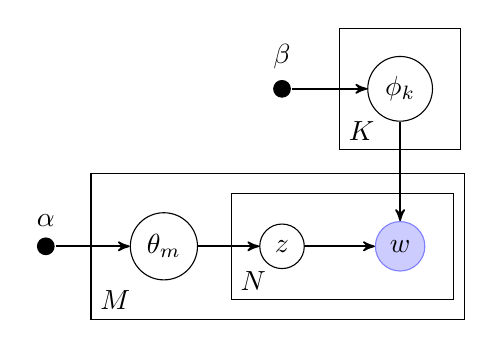
\begin{tikzpicture}
    [
      observed/.style={minimum size=15pt,circle,draw=blue!50,fill=blue!20},
      unobserved/.style={minimum size=15pt,circle,draw},
      hyper/.style={minimum size=1pt,circle,fill=black},
      post/.style={->,>=stealth',semithick},
    ]

    \node (w-j) [observed] at (0,0) {$w$};
    \node (z-j) [unobserved] at (-1.5,0) {$z$};  
    \node (z-prior) [unobserved] at (-3,0) {$\theta_m$};
    \node (z-hyper) [label=above:$\alpha$] at (-4.5,0) {};
    \filldraw [black] (-4.5,0) circle (3pt);
    \node (w-hyper) [label=above:$\beta$] at (-1.5,2.0) {};
    \filldraw [black] (-1.5,2.0) circle (3pt);
    
    \node (w-prior) [unobserved] at (0,2.0) {$\phi_k$};  
    
    \path
    (z-j) edge [post] (w-j)
    
    (z-hyper) edge [post] (z-prior)
    (z-prior) edge [post] (z-j)

    (w-hyper) edge [post] (w-prior)
    (w-prior) edge [post] (w-j)
    ;

    \node [draw,fit=(w-j) (z-prior), inner sep=14pt] (plate-context) {};
    \node [above right] at (plate-context.south west) {$M$};
    \node [draw,fit=(w-j) (z-j), inner sep=10pt] (plate-token) {};
    \node [above right] at (plate-token.south west) {$N$};
    
    \node [draw,fit=(w-prior), inner sep=10pt] (plate-context) {};
    \node [above right] at (plate-context.south west) {$K$};    

  \end{tikzpicture}
  \caption{Plate Diagram of LDA.}
  \label{fig:graphical-model}
\end{figure}

Above is what is known as a plate diagram of an LDA model where:
\begin{itemize}
\item $\alpha$ is the per-document topic distributions.
\item $\beta$ is the per-topic word distribution.
\item $\theta$ is the topic distribution for document m. $\theta_m$ is a discrete probability distribution over the topics, $\theta_m \sim \text{Dirichlet}(\alpha)$.
\item $\phi$ is the word distribution for topic $k$. $\phi_k$ is a discrete probability distribution over the vocabulary, $\phi_k \sim \text{Dirichlet}(\beta)$.
\item $z$ is the topic for the $n$-th word in document $m$.
\item $w$ is the specific word.
\end{itemize}

The objective function is to estimate $P(\theta, z, \phi | D, \alpha, \beta)$

\section{Gibbs sampling}
Suppose $\theta_1, \theta_2 \sim p(\theta_1, \theta_2)$
\begin{enumerate}
\item $\theta_{1}^{j} \sim p(\theta_1 | \theta_{2}^{(j-1)})$
\item $\theta_{2}^{j} \sim p(\theta_2 | \theta_{1}^{j})$
\end{enumerate}


\end{document}

